\documentclass[english]{beamer}
\usepackage[utf8]{inputenc}
\usepackage[T1]{fontenc}
\usepackage{amsfonts}
%\usepackage{amsthm}
\usepackage{makeidx}  % allows for indexgeneration
\usepackage{amsmath}
\usepackage{mathtools}
\usepackage{verbatim}
\usepackage{float}
\usepackage{graphicx}
\usepackage{times}  
%\usepackage[lined, boxed, linesnumbered]{algorithm2e}
\usepackage{array}
%\usepackage{makecell}
\usepackage{tikz}
\usepackage{lscape}
%\usepackage{caption}
%\usepackage{subcaption}
%\usepackage{subfig}

\beamertemplatenavigationsymbolsempty
\setbeamertemplate{footline}[frame number]

\usetheme{Antibes} % Beamer theme v 3.0
\usecolortheme{lily}

%\usebackgroundtemplate
%{
%  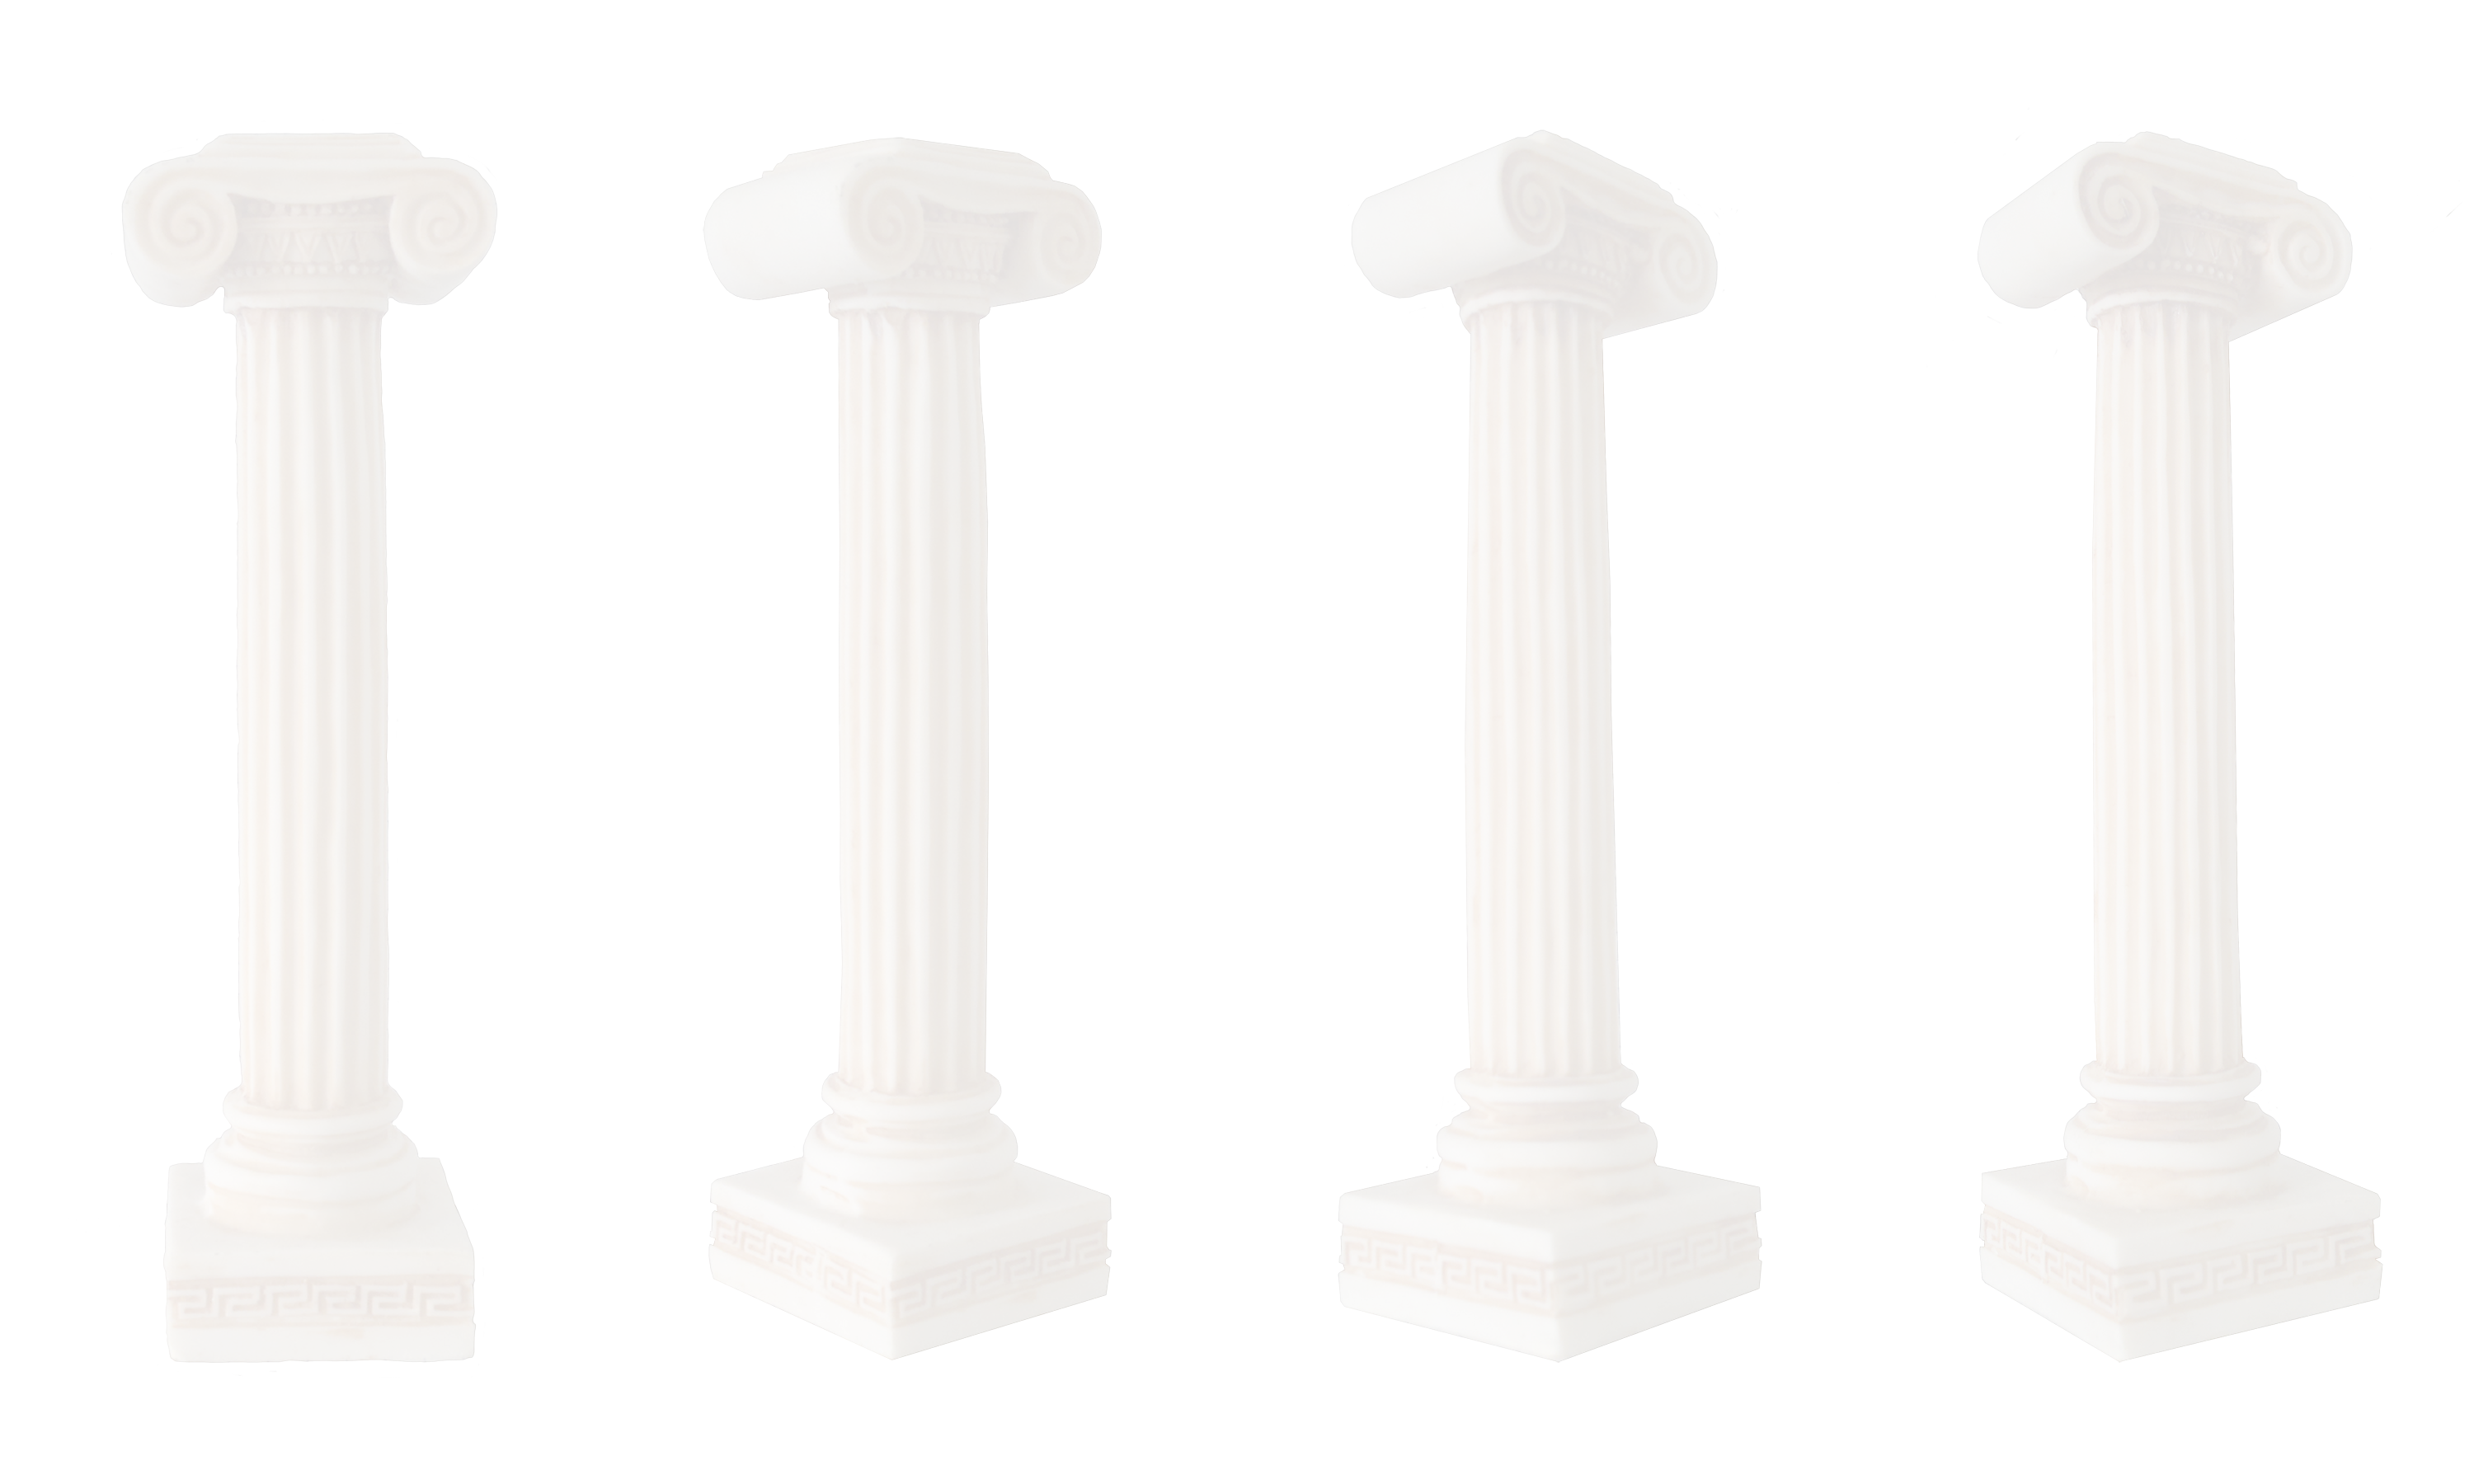
\includegraphics[width=\paperwidth,height=\paperheight]{columns.png}%
%}


\title{A Column Generation Approach for the Virtual Network Embedding Problem}
\author{Leonardo F.S. Moura and Luciana S. Buriol}
\date{December 8, 2014}
\institute{Computer Science Department, Federal University of Rio Grande do Sul\\Porto Alegre, Brazil}
%\newtheorem{proposition}{Proposition}
%\newtheorem{theorem}{Theorem}[section]
%\newtheorem{lemma}{Lemma}[section]
\begin{document}
\begin{frame}
\titlepage
\begin{figure}
    \centering
    
\includegraphics[scale=0.4]{inf.png}
\end{figure}
\end{frame}

%---------------------------
\section{Introduction}
%---------------------------
\begin{frame}
  \frametitle{Outline}
\begin{enumerate}
  \item Network Virtualization
  \item Virtual Network Embedding Problem
    \item Column Generation Algorithm
  \item Experimental Results and Conclusion
\end{enumerate}
\end{frame}
%---------------------------
\begin{frame}
  \frametitle{Network Virtualization}
Motivation
\begin{itemize}
  \item Hardware Heterogeneity
  \item Underutilization of resources
\end{itemize}
Network Virtualization
\begin{itemize}
  \item Began to gain traction in 2006
  \item Multiple virtual networks run on top of a physical network, sharing its resources.
\end{itemize}
Applications
\begin{itemize}
	\item Network Testbeds - New protocols can be tested without the need of 
     specialized hardware
	\item Cloud Computing - Client applications can share the same physical
      infrastructure.
\end{itemize}
\end{frame}
%---------------------------
\begin{frame}
\frametitle{Virtual Network Embedding Problem}
The main problem in Network Virtualization
\begin{columns}
\begin{column}{0.5\textwidth}
  \begin{figure}
    \centering
    \includegraphics[scale=0.4]{example.pdf}
    \caption{Example Instance}
  \end{figure}
\end{column}
\begin{column}{0.5\textwidth}
  \begin{figure}
    \centering
    \includegraphics[scale=0.32]{mapexample.pdf}
    \caption{Solution (cost = 50)}
  \end{figure}
\end{column}
\end{columns}
\end{frame}
%---------------------------
\begin{frame}
\frametitle{Virtual Network Embedding Problem}
\begin{itemize}
	\item State of the art
    \begin{itemize}
      \item NP-Hard
      \item Finding a feasible solution is NP-Hard
      \item Exact solutions are not widely studied in the literature
      \item Relaxation of ILP models for VNEP do not provide good lower bounds
    \end{itemize}
	\item This work
    \begin{itemize}
      \item Present a new Column Generation Model for the VNEP
      \item Better lower bounds than previous models
      \item To be embedded in a Branch \& Bound algorithm
    \end{itemize}
\end{itemize}
\end{frame}
%---------------------------
\begin{comment}
\begin{frame}
\frametitle{ILP Model}
{
\scriptsize
\begin{align}
     \min & \sum\limits_{(s,j) \in E^{S}} \sum\limits_{(v,w) \in E^{V}} B_{vw}~ y_{vwsj} & \nonumber \\
    s.t. & \sum\limits_{v \in V^{V}} C_{v} x_{vs} \leq C_{s}                                   & \forall s \in V^{S}  \label{eq:flowcap} \\
         & \sum\limits_{s \in V^{S}} x_{vs} = 1                                                & \forall v \in V^{V}  \label{eq:flowvirone}\\
         & \sum\limits_{v \in V^{V}} x_{vs} \leq 1                                             & \forall s \in V^{S} \label{eq:flowsubone} \\
         & \sum\limits_{j \in V^{S}} ( y_{vwsj} - y_{vwjs}) = x_{vs} - x_{ws} & \forall (v,w) \in E^{V}, s \in V^{S} \label{eq:flowflow} \\
         & \sum\limits_{(v,w) \in E^{V}} B_{vw}  y_{vwsj} \leq B_{sj}                 & \forall (s,j) \in E^{S} \label{eq:flowbandwidth} \\
         & x_{vs} \in \{0,1\}                                                         & \forall v \in V^{V}, s \in V^{S} \\
         & y_{klmn} \in \{0,1\}                                                         & \forall (k,l) \in E^{V}, (m,n) \in E^{S}
\end{align}
}
\end{frame}
\end{comment}
%---------------------------
\begin{frame}
  \frametitle{Two-phases algorithm}
  \begin{figure}
    \centering
    \includegraphics[scale=0.35]{example.pdf}
    \caption{Example Instance}
  \end{figure}
\end{frame}
%---------------------------
\begin{frame}
\frametitle{One-phase mapping}
\begin{columns}
\begin{column}{0.35\textwidth}
  \begin{figure}
    \centering
    \includegraphics[scale=0.35]{example.pdf}
    \caption{Example Instance}
  \end{figure}
\end{column}
\begin{column}{0.45\textwidth}
  \begin{figure}
    \centering
    \includegraphics[scale=0.35]{aux.pdf}
    \caption{Auxiliary Graph}
  \end{figure}
\end{column}
\end{columns}
\end{frame}
%---------------------------
\begin{frame}
\frametitle{One-phase algorithm}
\begin{columns}
\begin{column}{0.35\textwidth}
  \begin{figure}
    \centering
    \includegraphics[scale=0.35]{example.pdf}
    \caption{Example Instance}
  \end{figure}
\end{column}
\begin{column}{0.45\textwidth}
  \begin{figure}
    \centering
    \includegraphics[scale=0.35]{aux2.pdf}
    \caption{Auxiliary Graph}
  \end{figure}
\end{column}
\end{columns}
\end{frame}
%---------------------------
\begin{frame}
\frametitle{CG Model}
{
\begin{columns}
\begin{column}{0.35\textwidth}
  \begin{itemize}
    \item $x_{v,s}$ - virtual node $v$ is mapped into physical node $s$.
    \item $z_{p}$ - path $p$ is used
  \end{itemize}
\end{column}
\begin{column}{0.45\textwidth}
\tiny
\begin{align}
  \min  & \sum\limits_{k \in E^{V}}\sum\limits_{p \in P^k}  c_{p} B_k z_{p} \nonumber \\
        & \sum\limits_{s \in V^{S}} x_{v,s} = 1                                  & \forall v \in V^{V} \nonumber  \\
        & \sum\limits_{v \in V^{V}} x_{v,s} \leq 1                               & \forall s \in V^{S} \nonumber \\
        & \sum\limits_{p \in P^{k}} z_{p} = 1                                    & \forall k \in E^{V} \nonumber \\
        & \sum\limits_{k \in E^{V}}\sum\limits_{p \in P^{k}} \delta_{e,p} B_{k} z_{p} \leq B_{e} & \forall e \in E^{S} \nonumber \\
        &  \sum\limits_{k \in E^{V}}\sum\limits_{p \in P^k : (v,s) \in p} z_{p} \leq M x_{v,s} & \forall v \in V^{V}, s \in V^{S} \nonumber\\
        & 0 \leq x_{v,s} \leq 1  & \forall v \in V^{V}, s \in V^{S} \nonumber \\
        & 0 \leq z_{p}   \leq 1  & \forall p \in {P} \nonumber
\end{align}
\end{column}
\end{columns}
  Based on \cite{hu:2013}
}
\end{frame}
%---------------------------
\section{Column Generation Algorithm}
\begin{frame}
  \frametitle{Column Generation Algorithm (outline)}
\begin{enumerate}
	\item Find an initial set of columns
	\item Solve Restricted Master Problem
	\item Solve pricing problem
	\item If no columns are found, terminate, otherwise add new columns to RMP and goto~2
\end{enumerate}
\end{frame}
%---------------------------
\begin{frame}
\frametitle{Pricing}
%\begin{align}
%  r_{p} = \sum\limits_{e \in p : e \in E^S} B_{k} (1 - y_{e}) - \sum\limits_{(v,s) \in p : (v,s) \notin E^S} \pi_{v,s} - \lambda_{k} \nonumber
%\end{align}
  Find column with the smallest reduced cost

  \begin{figure}
    \centering
    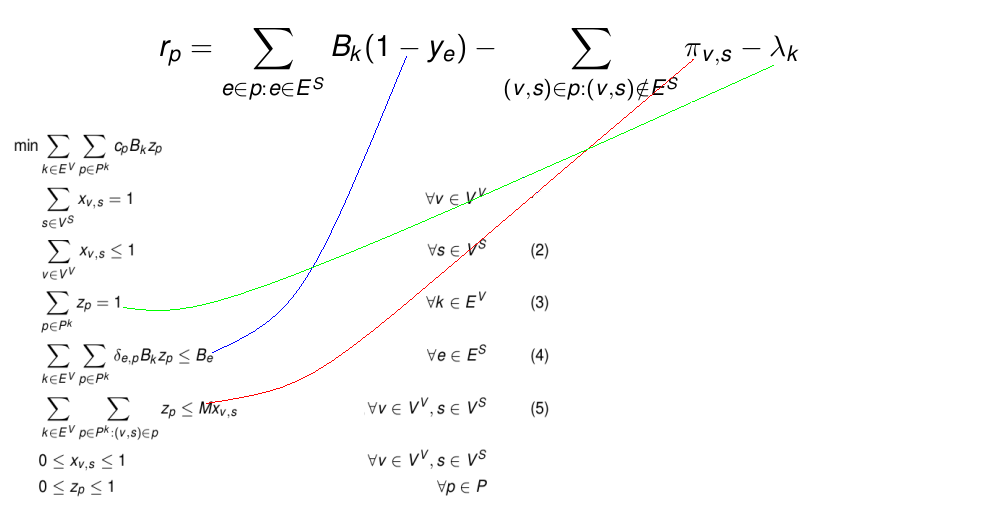
\includegraphics[scale=0.4]{redcost1.png}
  \end{figure}

\end{frame}
\begin{frame}
\frametitle{Pricing}
%\begin{align}
%  r_{p} = \sum\limits_{e \in p : e \in E^S} B_{k} (1 - y_{e}) - \sum\limits_{(v,s) \in p : (v,s) \notin E^S} \pi_{v,s} - \lambda_{k} \nonumber
%\end{align}
  The cost of a path in a graph is its reduced cost

  \begin{figure}
    \centering
    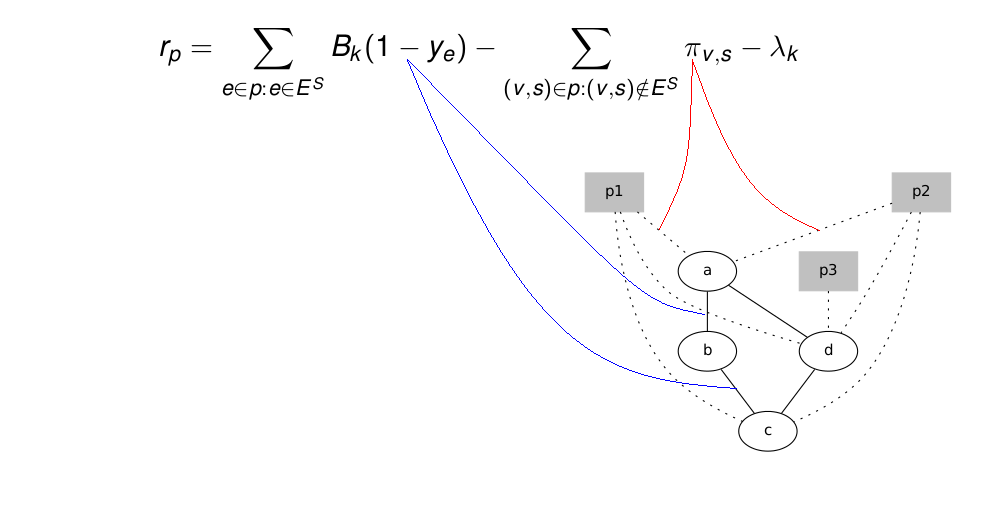
\includegraphics[scale=0.4]{redcost2.png}
  \end{figure}

\end{frame}
%---------------------------
\begin{frame}
\frametitle{Pricing}
  \begin{figure}
    \centering
    \includegraphics[scale=0.4]{subprob1.pdf}
    \caption{cost = 2}
  \end{figure}
\end{frame}
%---------------------------
\begin{frame}
\frametitle{Pricing}
  \begin{figure}
    \centering
    \includegraphics[scale=0.4]{subprob2.pdf}
    \caption{cost = 3}
  \end{figure}
\end{frame}
%---------------------------
\begin{frame}
\frametitle{Pricing}
  \begin{figure}
    \centering
    \includegraphics[scale=0.4]{subprob3.pdf}
    \caption{cost = 21}
  \end{figure}
\end{frame}
%---------------------------
\section{Column Generation Algorithm}
\begin{frame}
\frametitle{Column Generation Algorithm}
\begin{enumerate}
	\item Find an initial set of columns
	\item Solve Restricted Master Problem
	\item Build auxiliary graph
	\item For each virtual link $k$
	\item \quad If there exists a path in the auxiliary graph with negative cost, add column to the model
	\item end if no paths were found in this iteration, otherwise goto~2
\end{enumerate}
\end{frame}
%---------------------------
\section{Results}

\begin{frame}
\frametitle{Experimental Approach}
\begin{itemize}
  \item The CG algorithm bounds are compared with the optimal solution obtained with the ILP model solved using CPLEX.

  \item Two sets of random instances were generated:
    \begin{itemize}
      \item Set 1 - abundant resources
      \item Set 2 - scarce resources
    \end{itemize}
  %\item All tests were performed on processor Intel Core i7 930 with 12~Gb of memory. 
  %\item The commercial solver CPLEX 12.5 was used to solve the relaxed and integer models. 
  %\item All instances were generated using the GTI-ITM tool
  
  %\item ``Since network virtualization is an emerging field, the actual characteristics of substrate networks and VN requests are still not well understood'' \cite{Chowdhury2010}

\end{itemize}
\end{frame}
%---------------------------
\begin{frame}
\begin{table}[h]
\begin{center}
\scriptsize
  \begin{tabular}{c c | r | r r}
  \hline
  $|S|$&$|V|$&    GAP\%   & Time CG (s)    & Time ILP (s)         \\
  \hline
  10 & 2    &   0.00      &  0.01$\pm$0.00 &  0.01$\pm$0.00       \\
  20 & 2    &   0.00      &  0.01$\pm$0.00 &  0.02$\pm$0.00       \\
  40 & 2    &   0.00      &  0.01$\pm$0.00 &  0.04$\pm$0.01       \\
  80 & 2    &   0.00      &  0.01$\pm$0.00 &  0.21$\pm$0.05       \\
  10 & 4    &   10.20     &  0.01$\pm$0.00 &  0.05$\pm$0.03       \\
  20 & 4    &   6.77      &  0.01$\pm$0.00 &  0.12$\pm$0.05       \\
  40 & 4    &  0.00       &  0.01$\pm$0.00 &  0.37$\pm$0.17       \\
  80 & 4    &   0.00      &  0.01$\pm$0.00 &  3.17$\pm$0.92       \\
  20 & 8    &   0.10      &  0.01$\pm$0.00 &  0.92$\pm$0.88       \\
  40 & 8    &   4.48      &  0.01$\pm$0.00 &  10.84$\pm$10.32     \\
  80 & 8    &   0.00      &  0.01$\pm$0.00 &  887.92$\pm$43.36    \\
  40 & 16   &   20.19     &  0.02$\pm$0.00 &  594.58$\pm$86.23    \\
  \hline                                                                                  
  10 & 2    &   0.00      &  0.00$\pm$0.00 &  0.01$\pm$0.00       \\
  20 & 2    &   0.00      &  0.00$\pm$0.00 &  0.02$\pm$0.00       \\
  40 & 2    &   0.00      &  0.00$\pm$0.00 &  0.03$\pm$0.00       \\
  80 & 2    &   0.00      &  0.01$\pm$0.00 &  0.18$\pm$0.04       \\
  20 & 4    &   7.23      &  0.00$\pm$0.00 &  0.08$\pm$0.06       \\
  40 & 4    &  0.00       &  0.00$\pm$0.00 &  0.26$\pm$0.23       \\
  80 & 4    &   5.79      &  0.01$\pm$0.00 &  2.56$\pm$2.48       \\
  40 & 8    &  5.68       &  0.00$\pm$0.00 &  0.96$\pm$0.34       \\
  80 & 8    &  16.24      &  0.01$\pm$0.01 &  10.32$\pm$10.42     \\
\end{tabular}
\end{center}
\end{table}
\end{frame}
%---------------------------
\begin{frame}
\frametitle{Extensions}
\begin{itemize}
  \item In an extended work, the proposed CG model was embedded in a Branch \& Price algorithm
  \item Tested with larger instances and different topologies (random-sparse, random-dense, transit-stub, hierarchical)
\end{itemize}
\begin{columns}
\begin{column}{0.5\textwidth}
  \begin{figure}
    \centering
    \includegraphics[scale=0.3]{cost_fdensevir1.pdf}
  \end{figure}
\end{column}
\begin{column}{0.5\textwidth}
  \begin{figure}
    \centering
    \includegraphics[scale=0.3]{opt_fdensevir1.pdf}
  \end{figure}
\end{column}
\end{columns}
\end{frame}
%---------------------------
\section{Conclusion}
\begin{frame}
\frametitle{Conclusions}
Contribution
\begin{itemize}
	\item New CG model for VNEP with single-paths
	\item A good quality lower bound is obtained in a timely fashion
  \item Branch \& Price algorithm is able to solve larger instances than CPLEX
\end{itemize}
\end{frame}
%---------------------------
\begin{frame}
\frametitle{}
\huge
{ \center Thank you - muchas gracias }
\begin{figure}
    \centering
    
\includegraphics[scale=0.4]{inf.png}
\end{figure}
\end{frame}
\begin{frame}[allowframebreaks]
\bibliographystyle{apalike}
\bibliography{VNE}
\end{frame}
\end{document}



%---------------------------
\begin{frame}
\frametitle{teste}

\end{frame}

